\documentclass{article}
\usepackage{graphicx} % Required for inserting images
\usepackage{amsmath}
\usepackage{float}
\usepackage{textgreek}
\usepackage{siunitx}

\title{PHY 338K Lab Report 1}
\author{Lily Nguyen with Anna Grove}
\date{September 15, 2025}

\begin{document}

\maketitle

\section{Lab 1: Basic Measurements and Oscilloscope Use}

\subsection{Wiring inside the breadboard}

Using a digital multimeter in continuity mode, we tested which holes of the breadboard are internally connected. A diagram of the breadboard wiring is shown below.

\begin{figure}[h!]
    \centering
    \includegraphics[width=0.4\textwidth]{breadboard.png}
    \caption{Internal wiring of the breadboard.}
    \label{fig:breadboard}
\end{figure}

\subsection{Output impedance}

\subsubsection{Open circuit voltage}

With the circuit setup as in Figure 1-7, we set $V_{\text{in}}=+5 \text{ V}$ and measured the the open circuit output voltage. Using the DMM in DC mode, we got $V_{\text{OC}}=6.42\text{ V}$.

\subsubsection{Closed circuit current}

With the circuit setup as in Figure 1-8, we measured the short circuit output current by placing the DMM in series between $V_\text{out}$ and ground. We measured the short circuit current to be $I_{\text{SC}}=0.61 \text{ mA}$.

\subsubsection{Output impedance}

Using the measured open circuit voltage and short circuit current, we determined the output impedance of the circuit as

\begin{equation}
    Z_{\text{out}} = \frac{V_\text{OC}}{I_\text{SC}}
    = \frac{6.42 \,\text{V}}{0.00061 \,\text{A}}
    \approx 10.5 \,\text{k}\Omega
\end{equation}

\noindent This value is consistent with the resistance expected from the circuit setup. For resistor-only circuits, the output impedance is just the total resistance value.

\subsection{Voltage divider}

\subsubsection{Voltage divider circuit}

We constructed a voltage divider with two equal resistors and applied $V_\text{in}=5\text{ V}$. Using the voltage divider formula, we calculated

\begin{equation}
    V_\text{out}=V_\text{in}\frac{R_2}{R_1+R_2}=5\frac{9.93\si{\ohm}}{9.93\si{\ohm}+9.93\si{\ohm}}=2.50\text{ V}
\end{equation}

\noindent Our measured value was $V_\text{out}=3.207\text{ V}$. While the theoretical and measured results differ by about $0.71\text{ V}$, both values are of the correct order of magnitude. The discrepancy may be due to experimental error or limitations in the resistor tolerance.

\subsubsection{General case voltage divider}

For the general case, the voltage divider output is given by

\begin{equation}
    V_\text{out}=V_\text{in}\frac{R_2}{R_1+R_2}
\end{equation}

\noindent In the limit $R_2\gg R_1$, $V_\text{out}$ approaches $V_\text{in}$, meaning nearly the full input voltage appears across $R_2$. In the opposing limit $R_2\ll R_1$, $V_\text{out}$ approaches $0$, meaning nearly all the voltage drops across $R_1$. Physically, when $R_2$ is very large, it behaves almost like an open circuit, so nearly all the voltage drops across it. On the other hand, when $R_2$ is very small, it acts kind of like a short to ground, causing the output voltage to go to zero.

\subsection{Measuring voltage waveforms with an oscilloscope}

\subsubsection{Measuring the waveform from a function generator}

We connected the function generator output to Channel 1 of the oscilloscope and set it to produce a $1\text{kHz}$ sine wave. We attached the \SI{50}{\ohm} at the scope input and measured the frequency to be $f=1.043\text{ kHz}$ and peak-to-peak voltage to be $V=692\text{ mV}$. Without the terminator, we measured the frequency to be $f=1.045\text{ kHz}$ and the peak-to-peak voltage to be $V=1.384\text{ V}$.\\

\begin{figure}[H]
    \centering
    \includegraphics[width=0.47\textwidth]{"with terminator.png"}
    \hfill
    \includegraphics[width=0.47\textwidth]{"without terminator.png"}
    \caption{Oscilloscope display of a 1 kHz sine wave with (left) and without (right) a 50~$\Omega$ terminator.}
    \label{fig:scope_comparison}
\end{figure}

\noindent The difference occurs because the function generator has a \SI{50}{\ohm} internal output impedance. When the external \SI{50}{\ohm} terminator is added, it forms a voltage divider with internal resistance, reducing the observed amplitude by about half. Without the terminator, the oscilloscope's high input impedance draws negligible current we are able to observe nearly the full voltage source.

\noindent We should think of the oscilloscope as a voltmeter since it measures the voltage difference across its input and not the current going through it.


\begin{figure}[H]
    \centering
    \includegraphics[width=0.45\textwidth]{circuit with terminator.png}
    \hfill
    \includegraphics[width=0.45\textwidth]{circuit without terminator.png}
    \caption{Circuit schematic of the function generator and oscilloscope connection with (left) and without (right) a \SI{50}{\ohm} terminator.}
    \label{fig:circuit_comparison}
\end{figure}


\subsubsection{Scope triggering}

When we set the trigger level within the amplitude range of the sine wave, the oscilloscope locked onto a consistent crossing point and displayed a stable waveform. However, when we moved the trigger level outside the signal's range, the scope was unable to synchronize to a valid trigger, thus rendering an unstable waveform.

\begin{figure}[H]
    \centering
    \includegraphics[width=0.85\textwidth]{trigger level sketch.jpeg}
    \caption{Sketch of oscilloscope traces showing a stable sine wave when the trigger level is within the signal range (left) and unstable displays when the trigger level is set above or below the waveform (middle and right).}
    \label{fig:my_label}
\end{figure}

\noindent When we switched the trigger source to the TTL output of the function generator, the sine wave remained stable as we adjusted the trigger level up and down. Even with the DC offset shifting the waveform above or below the trigger, the output did not become unstable. The advantage of TTL is that it provides a well-defined and consistent timing reference independent of the wave's amplitude or offset.

\subsubsection{Square wave}

With DC coupling, changing the DC offset shifted the entire square wave either up or down relative to ground. With AC coupling, the DC component was blocked and the waveform was centered around \SI{0}{\volt} regardless of offset.

\begin{figure}[H]
    \centering
    \includegraphics[width=0.5\textwidth]{DC offset.png}
    \caption{Sketch of oscilloscope display for a square wave with DC offset (shown in DC coupling) and AC coupling.}
    \label{fig:my_label}
\end{figure}

\subsubsection{Function generator output impedance}

We modeled the function generator as a sorce with an internal resistance $R_\text{out}$ in series with its output. By attaching different load resistors $R_\text{Load}$, we measured the corresponding $V_\text{out}$. From the voltage divider equation,

\begin{equation}
    V_\text{out}=V\cdot \frac{R_\text{Load}}{R_\text{out}+R_\text{Load}}
\end{equation}

we rearranged it to the linear form

\begin{equation}
    \frac{1}{V_\text{out}}=\frac{1}{V}+\frac{R_\text{out}}{V}\left( \frac{1}{R_\text{Load}}\right)
\end{equation}

\noindent Plotting $\frac{1}{V_\text{out}}$ versus $\frac{1}{R_\text{Load}}$ gave a straight line. From the slope and intercept, we were able to extract the generator's internal resistance and open-circuit amplitude.

\subsubsection{RMS amplitude}

The measured RMS values were much larger than the theoretical predictions (\SI{0.707}{V} for sine, \SI{0.577}{V} for triangle, and \SI{1.0}{V} for square with $2\text{V}_{pp}$. This discrepancy is likely due to the DMM's AC measurement method, which assumes a sinusoidal input instead of computing the true RMS value, though the results remained consistent across frequencies.

\subsubsection{RMS amplitude}

The measured RMS values were much larger than the theoretical predictions (\SI{0.707}{V} for sine, \SI{0.577}{V} for triangle, and \SI{1.0}{V} for square with $2\text{V}_{pp}$). This discrepancy is likely due to the DMM's AC measurement method, which assumes a sinusoidal input instead of computing the true RMS value, though the results remained generally consistent across frequencies.

\begin{table}[H]
    \centering
    \begin{tabular}{ | c c c c | }
        \hline
        Frequency & Sine & Triangle & Square \\
        \hline
        10 Hz   & 0.100 V & 0.120 V & 2.000 V \\
        1 kHz   & 1.980 V & 1.900 V & 2.020 V \\
        100 kHz & 2.060 V & 1.920 V & 2.040 V \\
        \hline
    \end{tabular}
    \caption{Measured RMS amplitudes of sine, triangle, and square waves at different frequencies (2 Vpp input).}
    \label{tab:rms_measurements}
\end{table}

\subsubsection{Rise time}

With the function generator set to a \SI{1}{\mega\hertz} square wave, we measured the rise time of the waveform using the oscilloscope's measurement tools. The time for the signal to rise from $10\%$ to $90\%$ of its maximum value was \SI{62.79}{\nano\second}, as shown in the figure below.

\begin{figure}[H]
    \centering
    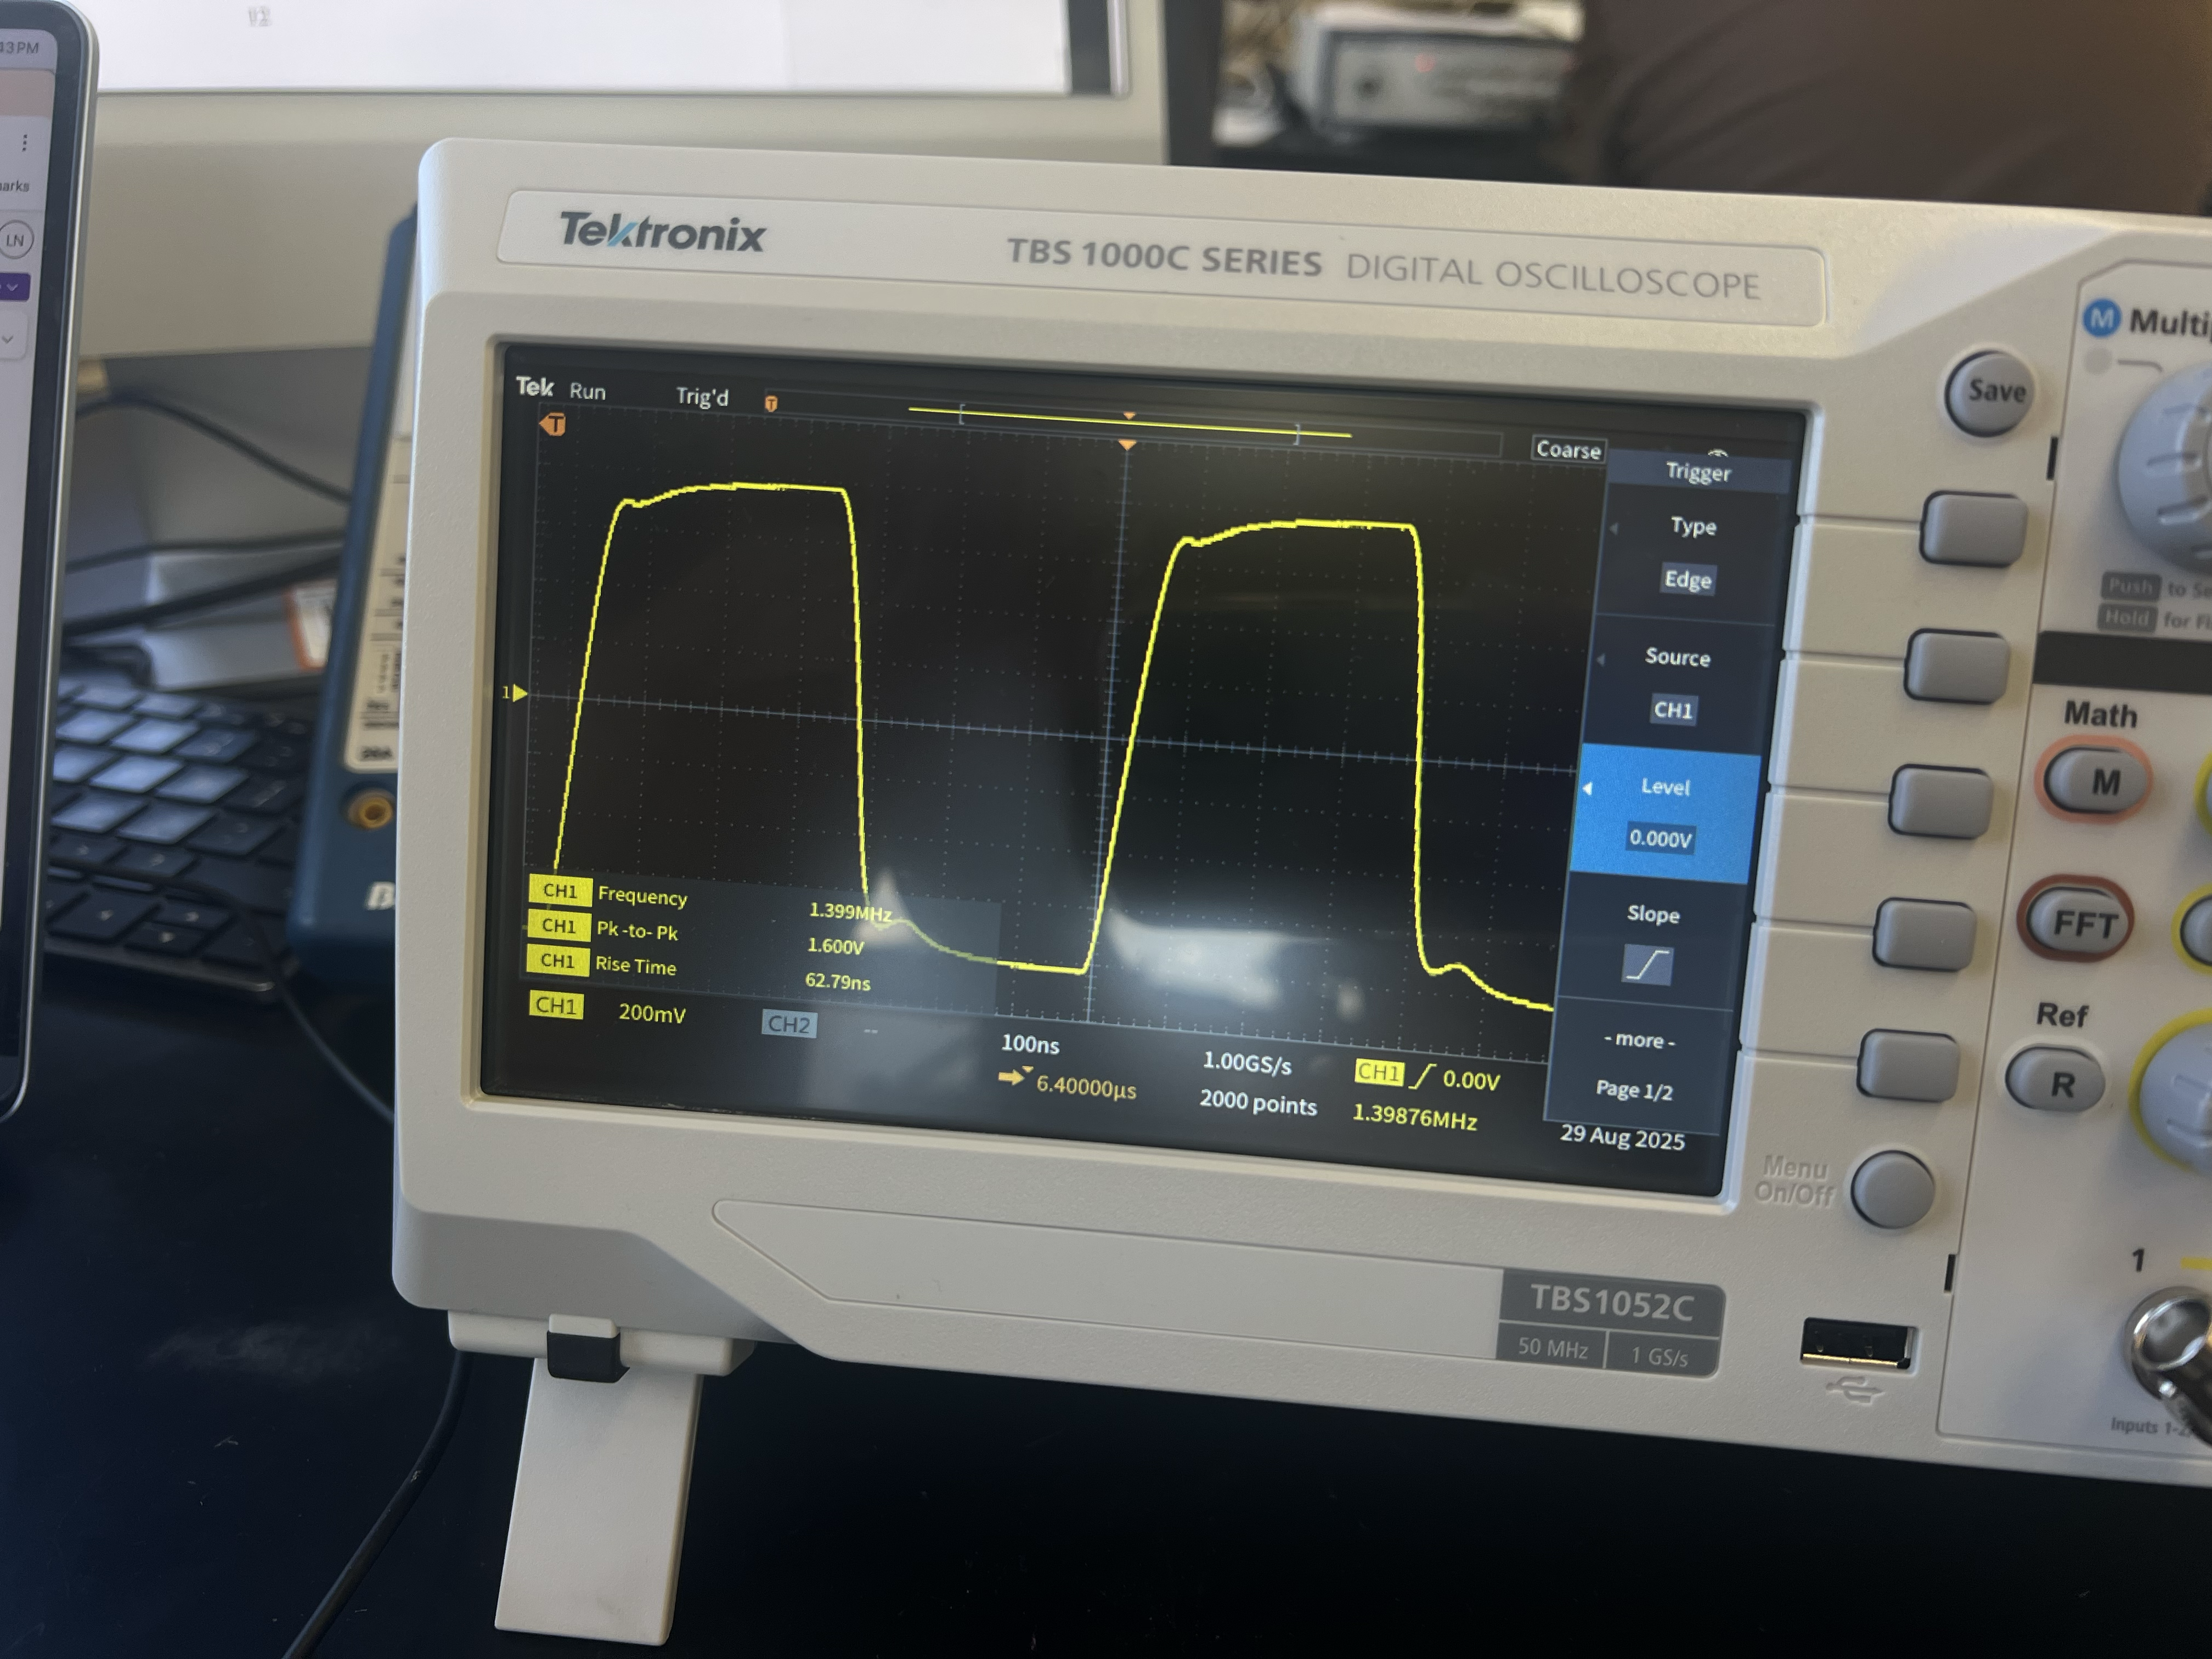
\includegraphics[width=0.5\textwidth]{rise time.png}
    \caption{Oscilloscope display of a \SI{1}{\mega\hertz} square wave showing the measured rise time of \SI{62.79}{\nano\second}.}
    \label{fig:rise_time}
\end{figure}


\section{Lab 2: RC Circuits}

\subsection{Circuit A}

\subsubsection{Rise and fall time}

To determine the time constant $\tau$ of an RC circuit, we measured the rising edge of the output waveform produced by a square wave input. We plotted the oscilloscope trace using Python and overlaid a horizontal line at \SI{1.04}{\volt}, which corresponds to one time constant after the waveform begins rising based on the formula

\begin{equation}
    V(t)=V_0 e^{-t/\tau}
\end{equation}

\noindent where $\tau=RC$.

With $V_\text{lower}=\SI{-4.04}{\volt}$ and $V_\text{upper}=\SI{3.96}{\volt}$, we have


\begin{figure}[H]
    \centering
    \includegraphics[width=0.9\textwidth]{2-1a.png}
    \caption{waveform}
    \label{fig:rise and fall time}
\end{figure}


*WORK ON THE REST OF LAB 2 LATER

\subsubsection{Integrator}

\subsubsection{Low-pass filter}

\subsection{Circuit B}

\subsubsection{Time constants}

\subsubsection{Differentiator}

\subsubsection{High-pass filter}

\subsection{Comparison with theory}

\subsubsection{Circuit A}

\subsubsection{Circuit B}

\section{Lab 3: Inductors and LC Filter Circuits}

\subsection{Impedance measurement with the LCR meter}

We used a Bourns RL181S-102J-RC inductor to observe how its impedance characteristics change with frequency. We measured the inductor's properties at four different frequencies (\SI{100}{\hertz}, \SI{1}{\kilo\hertz}, \SI{10}{\kilo\hertz}, and \SI{100}{\kilo\hertz}) using an LCR meter. We obtained the series inductance $L_S$, quality factor $Q$, equivalent series resistance (ESR), and phase angle $\theta$. The results are summarized in the table below.

\begin{table}[H]
    \centering
    \begin{tabular}{|c|c|c|c|c|}
    \hline
    \text{Frequency} & $L_S$ (µH) & $Q$ & \text{ESR (Ω)} & $\theta$ (deg) \\
    \hline
    100 Hz   & 950.0   & 0.274  & 2.1   & 15.3  \\
    1 kHz    & 944.4   & 2.69   & 2.2   & 69.6  \\
    10 kHz   & 944.6   & 23.7   & 2.5   & 7.5   \\
    100 kHz  & 928.5   & 137.0  & 4.12  & 89.5  \\
    \hline
    \end{tabular}
    \caption{Measured inductor parameters (Bourns RL181S-102J-RC) at various frequencies.}
    \label{tab:inductor_measurements}
\end{table}

\noindent According to the manufacturer’s datasheet, the inductor has a nominal inductance of \SI{1000}{\micro\henry} with a tolerance of $\pm 5\%$, a minimum quality factor $Q = 70$ at \SI{50}{\kilo\hertz}, and a self-resonant frequency (SRF) of \SI{0.77}{\mega\hertz}. Our measured inductance values ranged from \SI{928.5}{\micro\henry} to \SI{950.0}{\micro\henry}, which are well within our expectations.\\

\noindent From our measured results, we observed that at low frequencies (\SI{100}{\hertz}), the inductor deviated significantly from ideal behavior, exhibiting a low quality factor ($Q$) and a small phase angle ($\theta$). As the frequency increased, the inductor's behavior approached that of an ideal inductor. $Q$ increased, $\theta$ approached \SI{90}{\degree}, and the ESR remained relatively low. The inductor behaved most ideally between \SI{10}{\kilo\hertz} and \SI{100}{\kilo\hertz}, where $Q$ was high and the phase angle was nearly \SI{90}{\degree}.

\noindent To verify the consistency of ESR and $Q$ values, we used the definition of quality factor,

\begin{equation}
    Q=\frac{\omega L_s}{\text{ESR}}
\end{equation}

\noindent At $f=$\SI{1}{\kilo\hertz}, using $L_S = \SI{944.4}{\micro\henry}$ and ESR = \SI{2.2}{\ohm}, we computed,

\begin{equation}
    Q=\frac{2\pi(1000)(944.4\times 10^{-6}}{2.2}\approx 2.70
\end{equation}

\noindent which matches the measured value of $Q = 2.69$ and confirms the consistency of our data.\\

\noindent We also measured the impedance characteristics of a \SI{100}{\nano\farad} ceramic capacitor using the same LCR meter across the same set of frequencies. The results are summarized in the table below.

\begin{table}[H]
    \centering
    \begin{tabular}{|c|c|c|c|c|}
    \hline
    \text{Frequency} & $C_S$ (nF) & $D$ & \text{ESR (Ω)} & $\theta$ (deg) \\
    \hline
    100 Hz   & 99.37  & 0.000 & n/a   & -90.0 \\
    1 kHz    & 99.33  & 0.000 & 0.20  & -90.0 \\
    10 kHz   & 99.28  & 0.000 & 0.06  & -90.0 \\
    100 kHz  & 99.31  & 0.001 & 0.02  & -90.0 \\
    \hline
    \end{tabular}
    \caption{Measured parameters for 100nF ceramic capacitor at various frequencies.}
    \label{tab:capacitor_measurements}
\end{table}

\noindent Across all frequencies, the measured capacitance remained pretty consistent around \SI{99.3}{\nano\farad}. The phase angle $\theta$ also stayed consistently at \SI{-90}{\degree}, suggesting nearly ideal capacitive behavior. The dissipation factor $D$ remained extremely low and the equivalent series resistance (ESR) decreased with increasing frequency, which is what we expected.\\

\noindent Comparing both components, the ceramic capacitor exhibited behavior much closer to an ideal capacitor than the inductor did to an ideal inductor. Its phase angle stayed the same at \SI{-90}{\degree} and the ESR was minimal across the entire frequency range. The dissipation factor $D$ being close to $0$ also indicates that nearly all the energy is stored and returned rather than dissipated as heat. The inductor, on the other hand, only approached ideal behavior at higher frequencies (\SI{10}{\kilo\hertz} and above).


\subsection{Impedance measurements with an oscilloscope}


\subsection{Notch filter}

\subsection{Second-Order butterworth Filter}


\section*{Acknowledgements}

We would like to thank our laboratory instructor, Dr. Heinzen, and our teaching 
assistant, Kyle Gable, for their guidance and support through these labs.Their 
assistance and feedback were invaluable in helping us understand the experimental 
procedures and circuit concepts. We also appreciate the department's laboratory 
facilities and equipment, which made these experiments possible.

\end{document}